\section{Multi-Scenario Implementation of GMO Model Based on Efficiency Evaluation}
% 两个标题均可，"Multi-Scenario Implementation..."更侧重模型的实际应用过程，"Demonstration of the Model's Applicability Across Multiple Scenarios"更强调验证模型的普适性，根据上下文选择前者更合适


\vspace{-0.5cm}%在\end{table}下加一行\vspace{-1cm} 其中-1的作用是缩短与下方文字距离的 切记！必须是负数

\subsection{Implementation to A Two-story Nursery}

For multi-floor scenarios, we maintain \( \alpha_c \approx 0.4 \, \text{m}^2/\text{s} \) and use the following settings:
- Strongly connected component: Each single floor forms a strongly connected component
- Inter-floor connection: Staircases link multiple floors into a large connected component
- Inter-floor edge length: Calculated as "current floor staircase → target floor staircase → target room"


% 插入两张图，左右排布
\begin{figure}[htbp]  % h表示此处，t表示页顶，b表示页底，p表示独立一页，控制浮动体位置
	\centering  % 图表居中对齐
	\subfigure[First Floor]{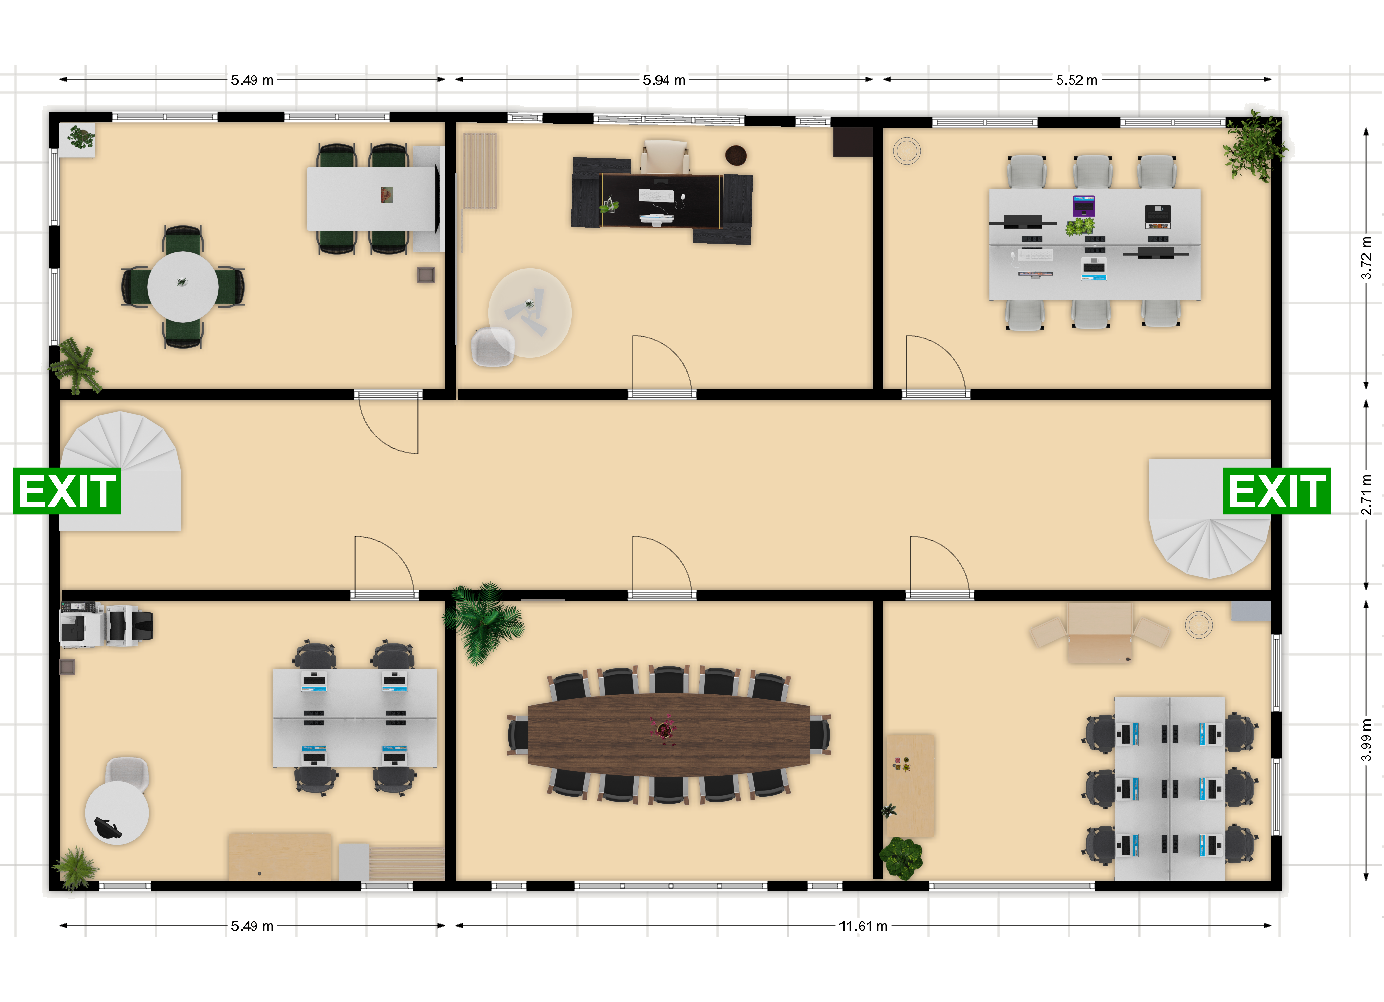
\includegraphics[width=.45\textwidth]{fig/layout21.png} % 注意图片名称或路径中不要有空格，否则会出错
      }
	\subfigure[Second Floor]{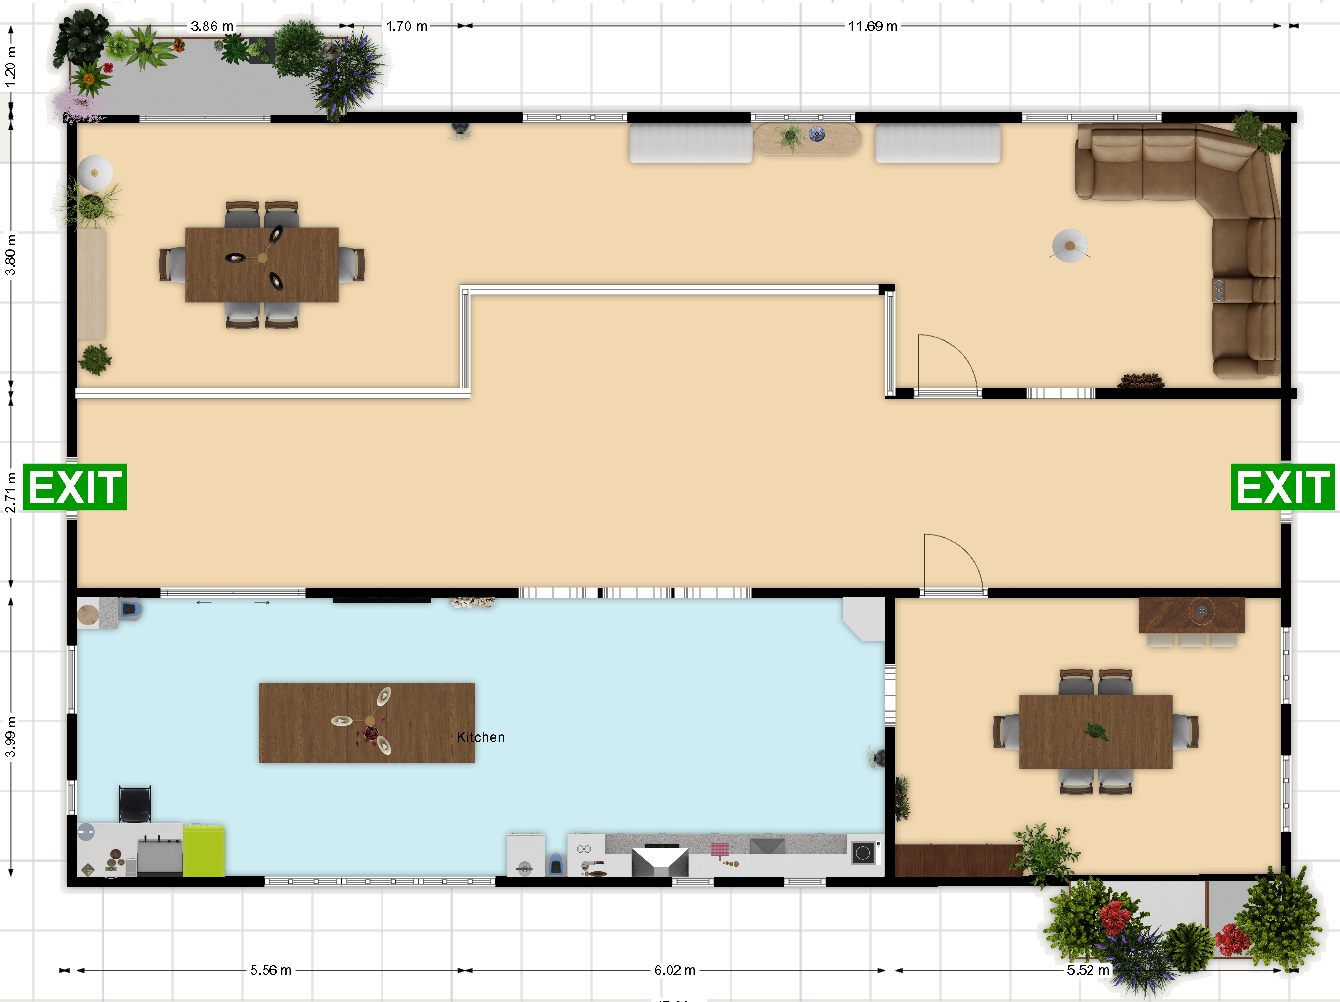
\includegraphics[width=.45\textwidth]{fig/layout22.png} % 注意图片名称或路径中不要有空格
      }
	\caption{Scheme for One-Story Office Building}
	\label{layout2}  % 为整个图表添加主标签，便于后续引用
\end{figure}
\vspace{-0.5cm}%在\end{table}下加一行\vspace{-1cm} 其中-1的作用是缩短与下方文字距离的 切记！必须是负数

The two-story nursery comprises a first-floor activity area and a second-floor rest area, connected by two spiral staircases. A corridor runs through the middle; there are two safety exits on both sides of the first floor, and spiral staircases on both sides of the second floor leading down to the first floor.

As shown in the floor plan (Figure \ref{layout2}) and the 3D diagram in the previous text (Figure \ref{fig:layoutpre}), we selected a two-story children's nursery to validate our model. Its first floor has 6 rooms with a layout similar to the office in the previous section, including 5 activity rooms and 1 craft room equipped with a large long table. The second floor features a kitchen with blue floor tiles, an adjacent dining area, and a large living room on the opposite side.

Table \ref{tab:room_parameters} presents our estimated search volumes ($Q$) for different rooms in this building.


\textbf{Floor Parameters}
\begin{table}[htbp]
	\begin{center}
		\caption{Room Parameters and Calculated $Q$ ($\text{m}^2$) Values}
		\begin{tabular}{c c c c c c c}
			\toprule[2pt]
			\multicolumn{1}{m{3cm}}{\textbf{Room Type}}
			&\multicolumn{1}{m{1.5cm}}{\textbf{Quantity}}
			&\multicolumn{1}{m{1.5cm}}{\textbf{ $A$ ($\text{m}^2$)}}
			&\multicolumn{1}{m{1cm}}{\textbf{ $ L$}}
			&\multicolumn{1}{m{1cm}}{\textbf{ $ C$}}
			&\multicolumn{1}{m{1cm}}{\textbf{ $ E$}}
			&\multicolumn{1}{m{2cm}}{\textbf{  $ Q$ ($\text{m}^2$)}}\\
			\midrule
			Activity Room & 5 & 30.00 & 1.2 & 1.2 & 1.3 & 61.78 \\
			Craft Room  & 1 & 73.72 & 1.4 & 1.3 & 1.5 & 248.47 \\
			Kitchen & 1 & 46.28 & 1.4 & 1.3 & 1.5 & 151.61 \\
			Dining Area & 1 & 36.91 & 1.1 & 1.2 & 1.3 & 69.67 \\
			Living Room & 1 & 45.59 & 1.0 & 1.1 & 1.2 & 36.19 \\
			\bottomrule[2pt]
		\end{tabular}\label{tab:room_parameters}		
	\end{center}
\end{table}



\begin{figure}[hbtp]
    \centering
    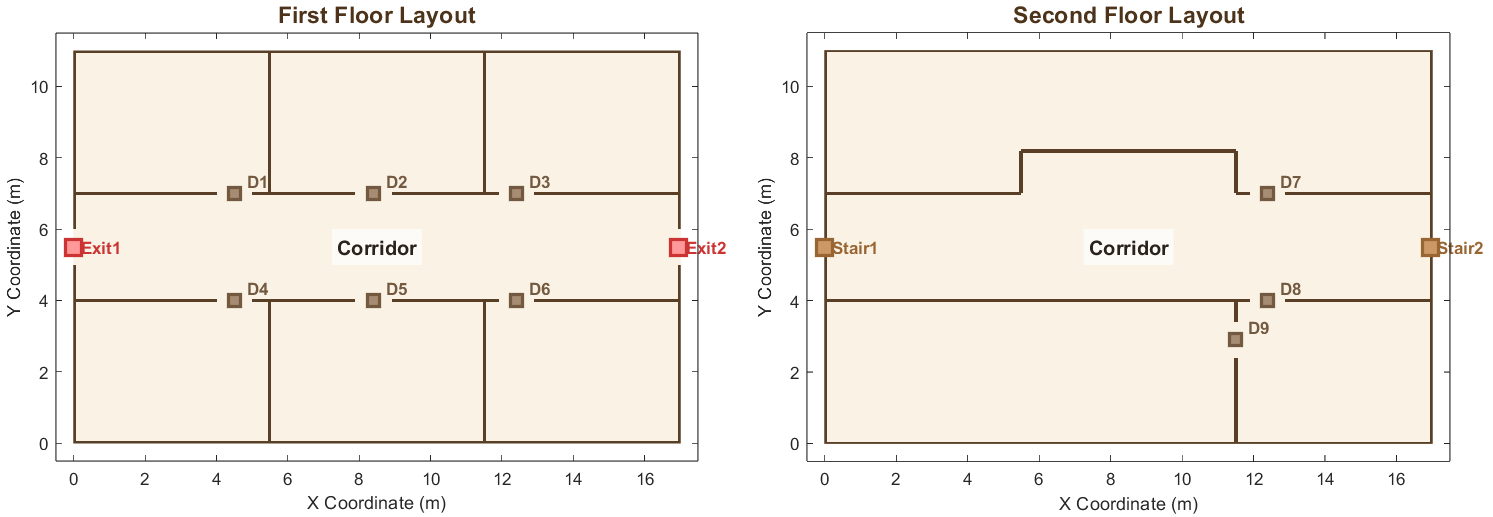
\includegraphics[width=0.75\textwidth]{fig/layout2.png} % 替换为实际图片路径
    \caption{Room Mask of the Building}
    \label{mask2}
\end{figure}

We programmed and drew room masks in the software based on the actual room layout, as shown in Figure \ref{mask}, to identify the positions of walls, safety exits, staircases, and room doors.

Then We calculated the distance for ascending and descending stairs using the inclination angle of 45° and the floor height. After abstracting room doorways as points, the Euclidean distance was used to calculate the spacing between connectable points, while the Manhattan distance was applied to points on the second floor.

Subsequently, the GA (Genetic Algorithm) and SA (Simulated Annealing) algorithms in the \textbf{GMO model} were employed to optimize the responders' paths.


However, our algorithm can actually assign any number of responders to search any number of rooms; we need to determine the optimal number of emergency responders.





\subsection{Efficiency-based Optimal Responser Quantity Evaluation}

To find the optimal number of responders, we developed a comprehensive evaluation system with a core scoring function: $S(n) = \alpha E_{\text{time}}(n) + \beta U(n) + \gamma B(n)$ . The weighting reflects that time efficiency is most critical in emergency response, resource utilization comes next, and load balancing also deserves consideration.

\textbf{Maximum Completion Time $T_{\text{max}}(n)$} represents the moment when the last firefighter finishes, determining the overall operation completion time, calculated as: $T_{\text{max}}(n) = \max_{j=1}^{n} \left( \sum_{i \in R_j} t_i \right)$ where $R_j$ is the set of rooms assigned to firefighter $j$. 

\textbf{Time per Room $T_{\text{room}}(n)$} shows the average search time per room, indicating work efficiency, defined as: $T_{\text{room}}(n) = T_{\text{total}}(n)/|R|$ where $T_{\text{total}}(n)$ is the total completion time across all firefighters: $T_{\text{total}}(n) = \sum_{j=1}^{n} \sum_{i \in R_j} t_i$ 

Both $T_{\text{max}}(n)$ and $T_{\text{room}}(n)$ are normalized and combined into the time efficiency score: $E_{\text{time}}(n) = w_1 \cdot \text{norm}(-T_{\text{max}}(n)) + w_2 \cdot \text{norm}(-T_{\text{room}}(n))$, which integrates key time metrics to evaluate overall temporal performance. 

\textbf{Utilization Rate $U(n)$} measures how efficiently human resources are used, calculated as the ratio of actual work done to theoretical capacity: $U(n) = |R|/\mathbb{E}[\text{assigned rooms}] = |R|/(n \cdot \text{average load})$ In our scenario, utilization remains at 100\% since there are always enough rooms to keep all firefighters busy.

\textbf{Load Balancing $B(n)$} evaluates how evenly tasks are distributed among team members; when workloads are balanced equally, the score is high, while significant disparities lower the score. Good load balancing ensures both team efficiency and prevents individual burnout, computed as: $B(n) = 1 - \sigma_T/\mu_T$ where $\sigma_T$ is the standard deviation of firefighters' working times, and $\mu_T$ is the average working time.

\begin{figure}[hbtp]
    \centering
    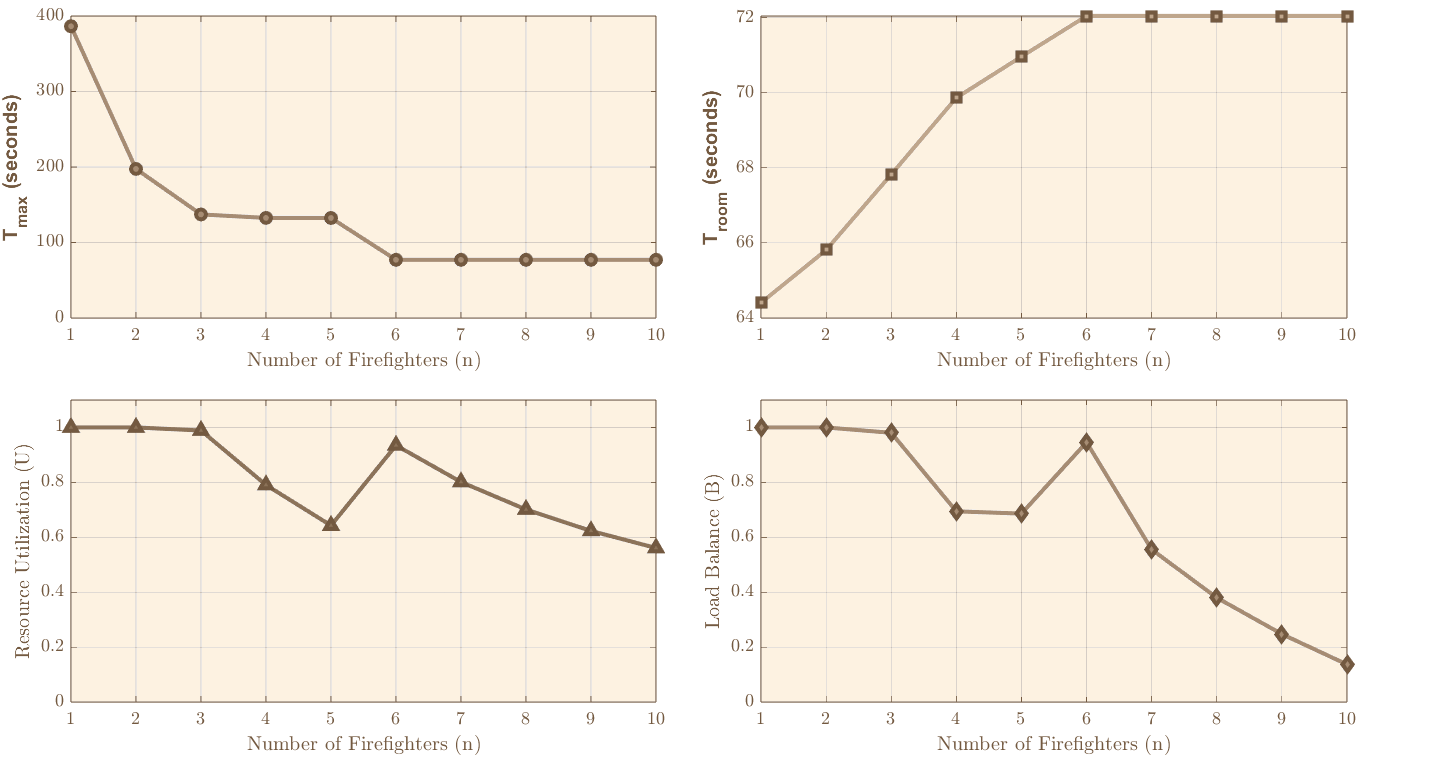
\includegraphics[width=0.8\textwidth]{fig/NumFireFighters.png} % 替换为实际图片路径
    \caption{Indicators Vary with the Number of Responders}
\end{figure}

Notably, our simulation of different team sizes revealed key performance trends. While more firefighters reduce $T_{\text{max}}$ through parallel work, $T_{\text{room}}$ may rise due to coordination overhead, and load balancing peaks at moderate team sizes.

Among specific configurations, with weight coefficients set as $\alpha = 0.5$, $\beta = 0.3$, $\gamma = 0.2$, comprehensive scoring shows that when considering all indicators holistically, the optimal number of firefighters is 3, which yields the highest comprehensive score $S(3) = \textbf{0.9326}$, presented in Figure \ref{3firefighters}.

\begin{figure}[hbtp]
    \centering
    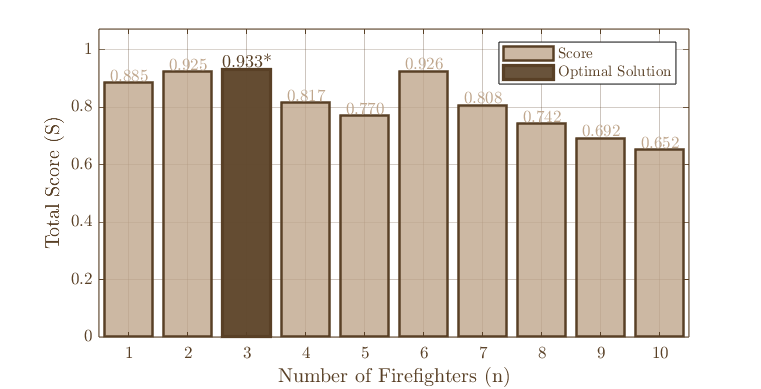
\includegraphics[width=0.75\textwidth]{fig/threeFireFighters.png} % 替换为实际图片路径
    \caption{Score of the Number of Responders}
    \label{3firefighters}
\end{figure}

This optimal solution underscores \textbf{balanced} decision-making in emergency response—prioritizing speed while ensuring rational resource use and equitable workloads. 

If more than the best number of responders are available, redundant resources should be fully utilized. For instance, extra responders can be assigned to communication and rescue coordination, with standby mobile teams ready to handle emergencies, sparing no effort to safeguard the lives of those at risk from unexpected incidents. 

If the number of responders is less than the optimal, the best path planning scheme for that specific number of personnel should be adopted for search and rescue operations. This approach also ensures maximum rescue efficiency, allowing every bit of rescue effort to function effectively in protecting lives.

Here, we use 3 responders to visually present the paths, as shown in Figure \ref{best2}. 

\begin{figure}[hbtp]
    \centering
    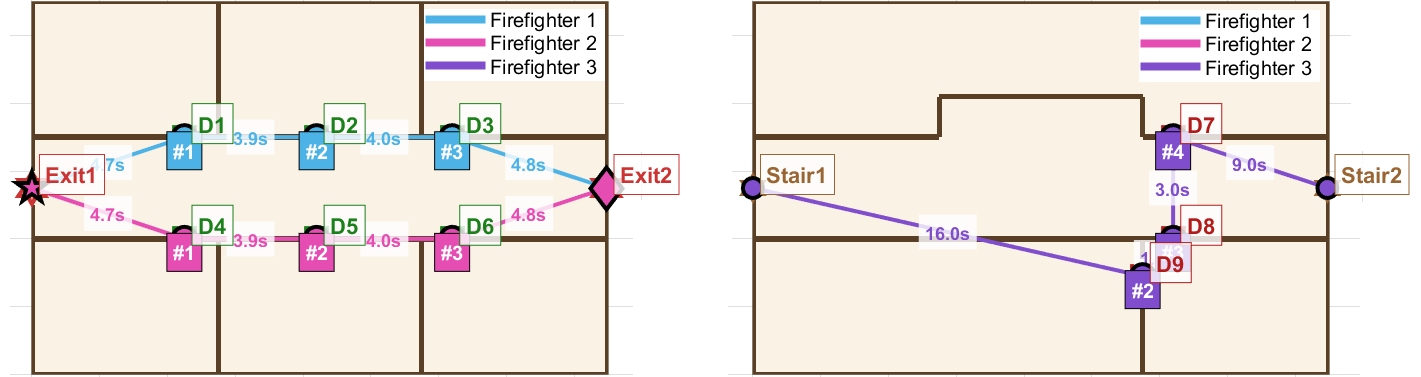
\includegraphics[width=0.75\textwidth]{fig/bestpath2.png} % 替换为实际图片路径
    \caption{The Best Scheme with 3 Responders}
    \label{best2}
\end{figure}

The minimum time required for all emergency responders to complete the search and rescue is as follows:

\begin{itemize}
    \item Responder 1: Total movement time: 17.4s; Search time ($T_{\text{check}}$): 113.4s; Total: 130.8s
    \item Responder 2: Total movement time: 17.4s; Search time ($T_{\text{check}}$): 90.6s; Total: 108.0s
    \item Responder 3: Total movement time: 13.5s; Search time ($T_{\text{check}}$): 120.1s; Total: 133.6s
\end{itemize}

Note that in this visualization, the connecting lines between two points do not represent actual paths but are for illustrative purposes only. The time labeled on the lines indicates the duration consumed by responders moving along the actual paths.


\subsection{Implementation to World Trade Center (WTC3)}


\begin{figure}
    \centering
    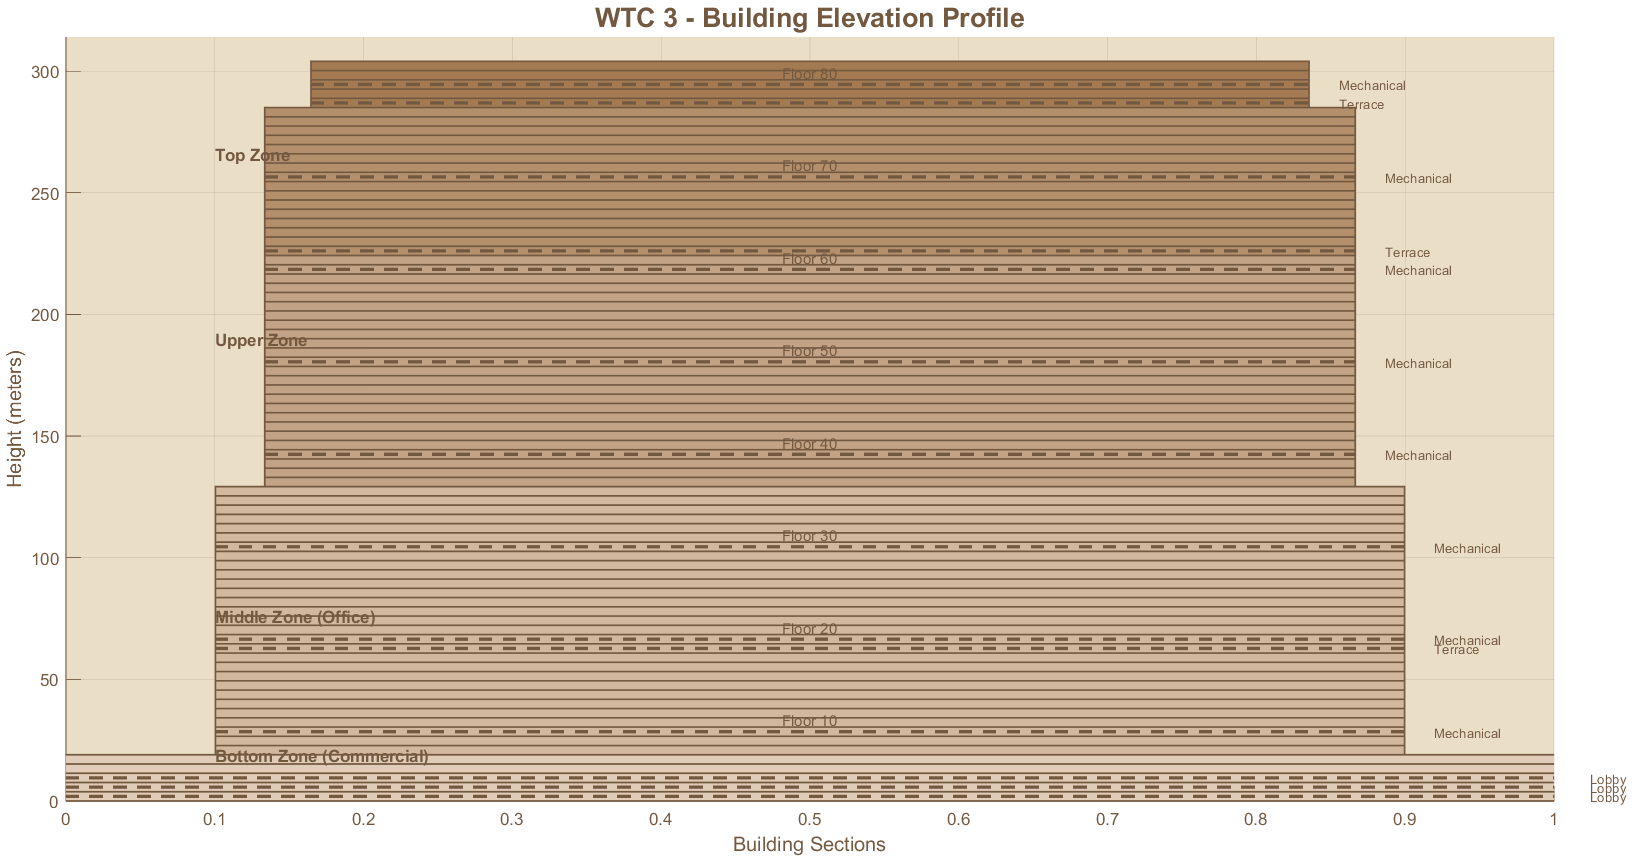
\includegraphics[width=0.95\linewidth]{fig/layout3.png}
    \caption{Enter Caption}
    \label{fig:layout3}
\end{figure}





%介绍布局Building Overview：太多了，可删减

The third WTC building has a height of 1079 feet (328 meters) and 80 floors, divided into four functional zones.

\subsection{Zone Parameters}
\subsubsection{Bottom Zone (1st to 5th Floors: Commercial Area)}
- Function: Retail space + trade layer (suitable for financial transactions)
- Entrances/exits: 9 (5 street-facing, 2 connected to transportation hubs, 2 linked to commercial complexes)
- Layout: Open circulation design, connected to subway and PATH train network
- Specifications:
  - Floor area: \( A \approx 6503 \, \text{m}^2 \) per floor
  - Ceiling height: 20 feet
  - Design: Column-free large-space
- Parameters: \( L = 1.3 \), \( C = 1.1 \), \( E = 1.0 \)

\subsubsection{Middle Zone (6th to 75th Floors: Office District)}
- Function: Standard office spaces
- Layout: Centered on reinforced concrete core, perimeter offices with 360° Manhattan views
- Specifications:
  - Ceiling height: 13 feet
  - Floor area (gradually tapering):
    - 35th-59th floors: \( A \approx 4087.6 \, \text{m}^2 \) per floor
    - 60th-75th floors: \( A \approx 3437.3 \, \text{m}^2 \) per floor
- Parameters: \( L = 1.2 \), \( C = 1.0 \), \( E = 1.0 \)

\subsubsection{Upper Zone (76th to 80th Floors)}
- Function: High-end office or specialized functions (flexible layout)
- Key feature: 76th floor with outdoor terrace
- Specifications:
  - Floor area: \( A \approx 2879.9 \, \text{m}^2 \) per floor (smallest in the building)
- Parameters: \( L = 1.2 \), \( C = 1.0 \), \( E = 1.0 \)

\subsubsection{Special Floors}
1. Outdoor terrace floors (17th, 60th, 76th):
   - \( A \approx 2879.9 \, \text{m}^2 \) per floor
   - Parameters: \( L = 1.5 \), \( C = 1.1 \), \( E = 1.0 \)
   - Requirements: Reserved terrace access points and protective facilities

2. Mechanical floors (8 floors total):
   - Function: Housing HVAC, electrical and other equipment (no regular usable space)
   - Layout: Centered on equipment rooms and piping
   - \( A \approx 464.5 \, \text{m}^2 \) per floor
   - Parameters: \( L = 1.6 \), \( C = 1.3 \), \( E = 1.0 \)

3. Three-story double-height lobby:
   - Height: Approximately 19 meters
   - Design: Black granite walls, white granite flooring (public reception area)
   - Total area: \( A \approx 950 \, \text{m}^2 \) (for 3 floors)
   - Parameters: \( L = 1.2 \), \( C = 1.0 \), \( E = 1.0 \)
   

\subsection{Feasibility Analysis of Simplified Path Optimization with Limited Responders}

When the number of responders is much smaller than the number of rooms, the approach of simplifying path optimization by prioritizing shortest path planning and then adding average search time is theoretically feasible, supported by the following key arguments:

\textbf{1. Dominance of Movement Time in Total Task Duration}
In scenarios with scarce responders, each responder must cover a large number of rooms. The total task duration consists of two components: inter-room movement time ($T_{\text{move}}$) and intra-room search time ($T_{\text{check}}$). When each responder is assigned numerous rooms, the cumulative movement time—affected by path layout, node distances, and routing efficiency—becomes the primary determinant of total duration. In contrast, $T_{\text{check}}$ tends to average out across multiple rooms due to the assumed uniform skill distribution of all responders. Thus, minimizing movement time through shortest-path planning has a more significant impact on optimizing total time than fine-tuning search time allocations.

\textbf{2. Insignificance of Individual Room Search Volumes}
The assumption that all responders follow the same skill distribution ensures consistent average search efficiency across rooms. When each responder is responsible for a large number of rooms, variations in individual room search volumes ($Q$) become negligible at the aggregate level. For example, a room with a slightly higher $Q$ will be offset by others with lower $Q$ in the same route, making the total search time for the route approximately equal to the number of rooms multiplied by the average $T_{\text{check}}$. This characteristic allows us to decouple path optimization from specific room volumes, focusing solely on minimizing movement distance.

\textbf{3. Computational Efficiency in High-Rise Building Scenarios}
For ultra-tall buildings with numerous floors and rooms (e.g., the 80-story third WTC building), complex mask-based path planning that accounts for detailed room parameters at every node faces substantial computational pressure. The simplified approach of "shortest path + average search time" reduces the dimensionality of the optimization problem—this not only accelerates algorithm convergence but also retains practical validity, as the core goal of minimizing total rescue time aligns with prioritizing movement efficiency.

In summary, when the number of responders is far fewer than the number of rooms, the proposed simplification balances accuracy and efficiency: shortest-path planning addresses the dominant component of total time, while averaging search time leverages the uniformity of responder skills and the law of large numbers, making it a reasonable and effective strategy.



% 插入两张图，左右排布
\begin{figure}[htbp]  % h表示此处，t表示页顶，b表示页底，p表示独立一页，控制浮动体位置
	\centering  % 图表居中对齐
	\subfigure[Heatmap of Distace of Nodes in WTC3]{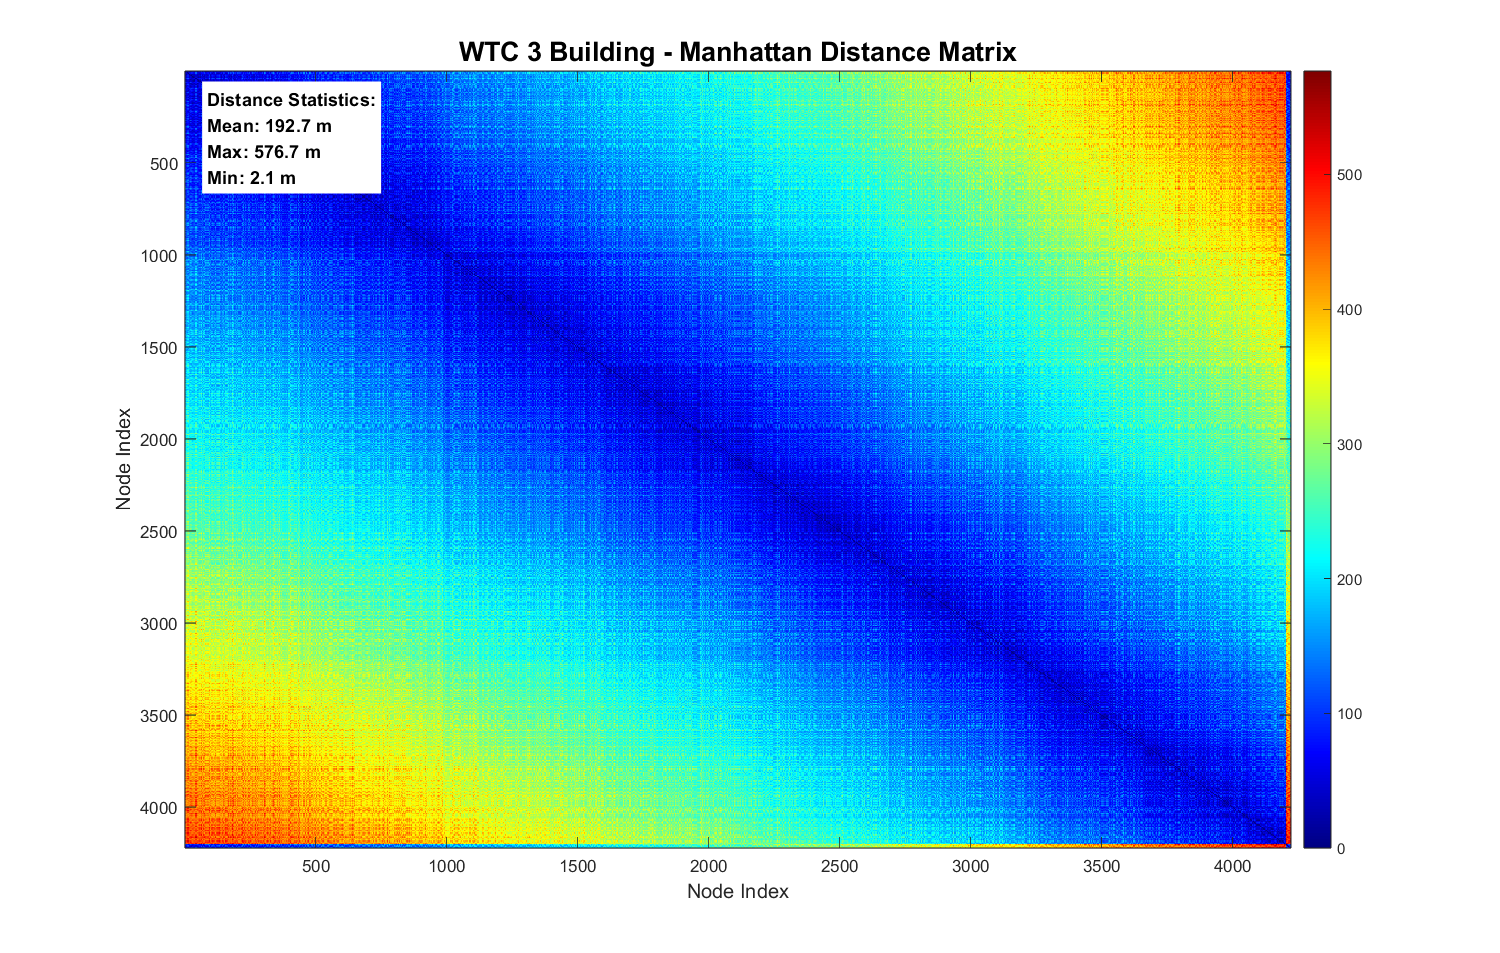
\includegraphics[width=.4\textwidth]{fig/wtc3ManhattanDistance.png} % 注意图片名称或路径中不要有空格，否则会出错
      }
	\subfigure[Best Scheme for 3 responders]{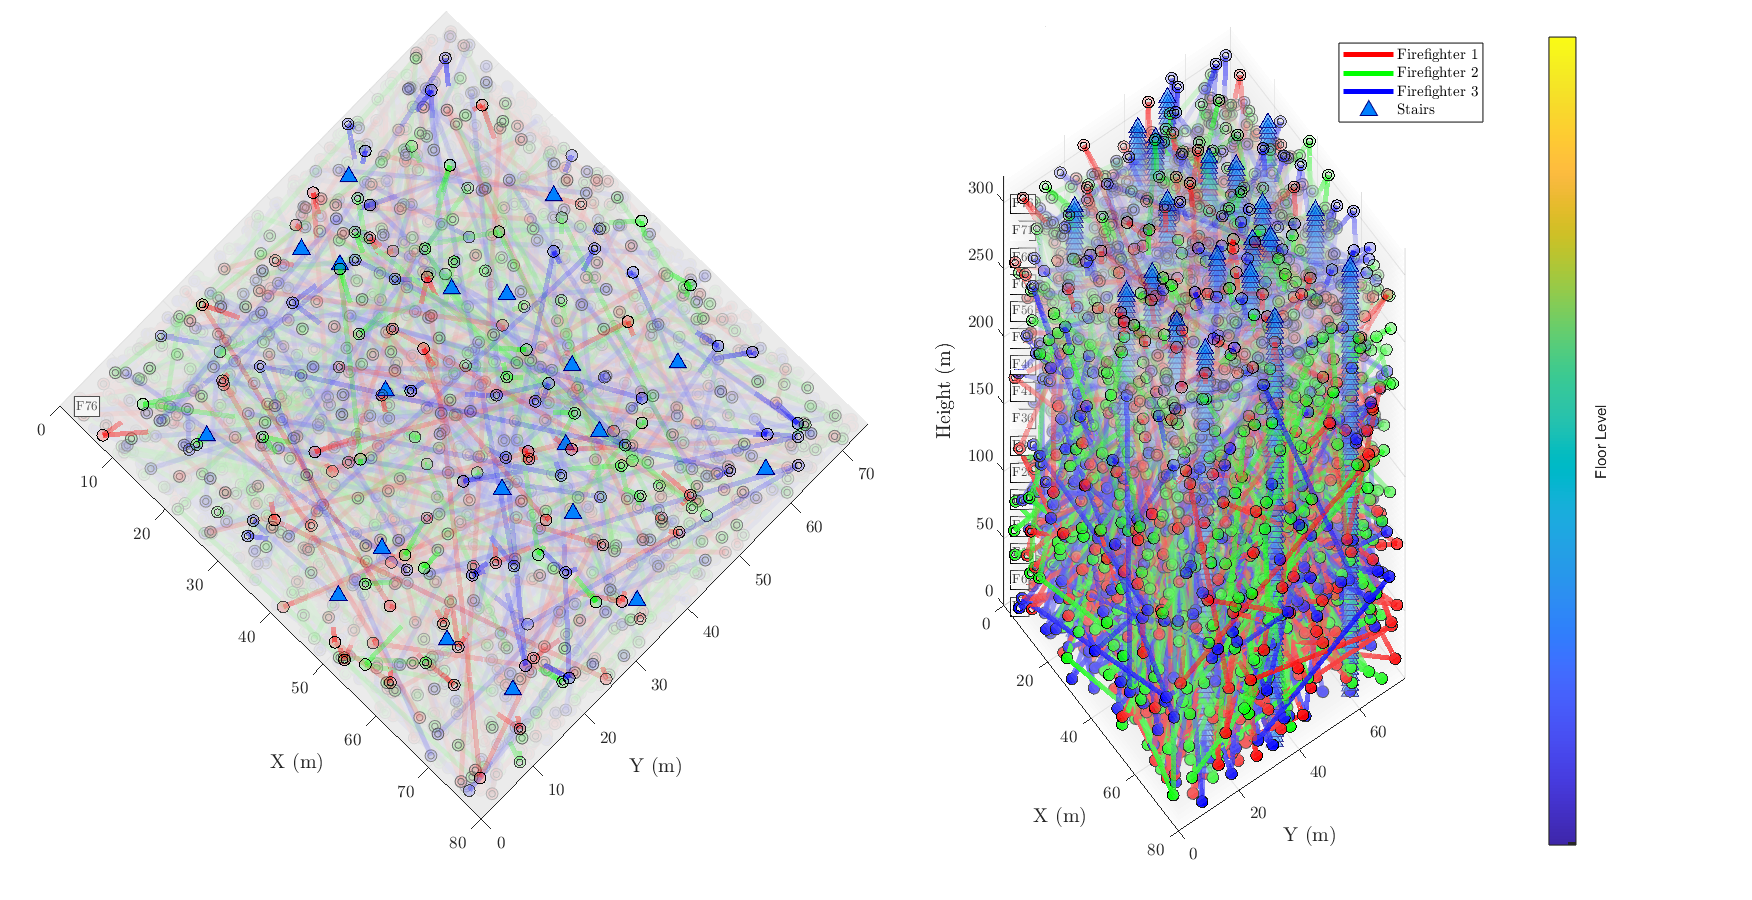
\includegraphics[width=.46\textwidth]{fig/wtc.png} % 注意图片名称或路径中不要有空格
      }
	\label{wtc}  % 为整个图表添加主标签，便于后续引用
\end{figure}
\vspace{-0.5cm}%在\end{table}下加一行\vspace{-1cm} 其中-1的作用是缩短与下方文字距离的 切记！必须是负数

For our algorithm, after calculating the Manhattan distance matrix heatmap between each pair of points, we incorporated it into the model and solved it using GA (Genetic Algorithm) and SA (Simulated Annealing) algorithms. Finally, in the Efficiency-based Optimal Responder Quantity Evaluation model, it is determined that the optimal number of firefighters for search and rescue is 15. The maximum time is calculated as \( T = \max(T_{\text{move}}) + \sum T_{\text{check}} / 15 \), which is approximately 20.4 minutes.

\subsection{Algorithm Performance Comparison (GA vs. SA)}
\begin{figure}
    \centering
    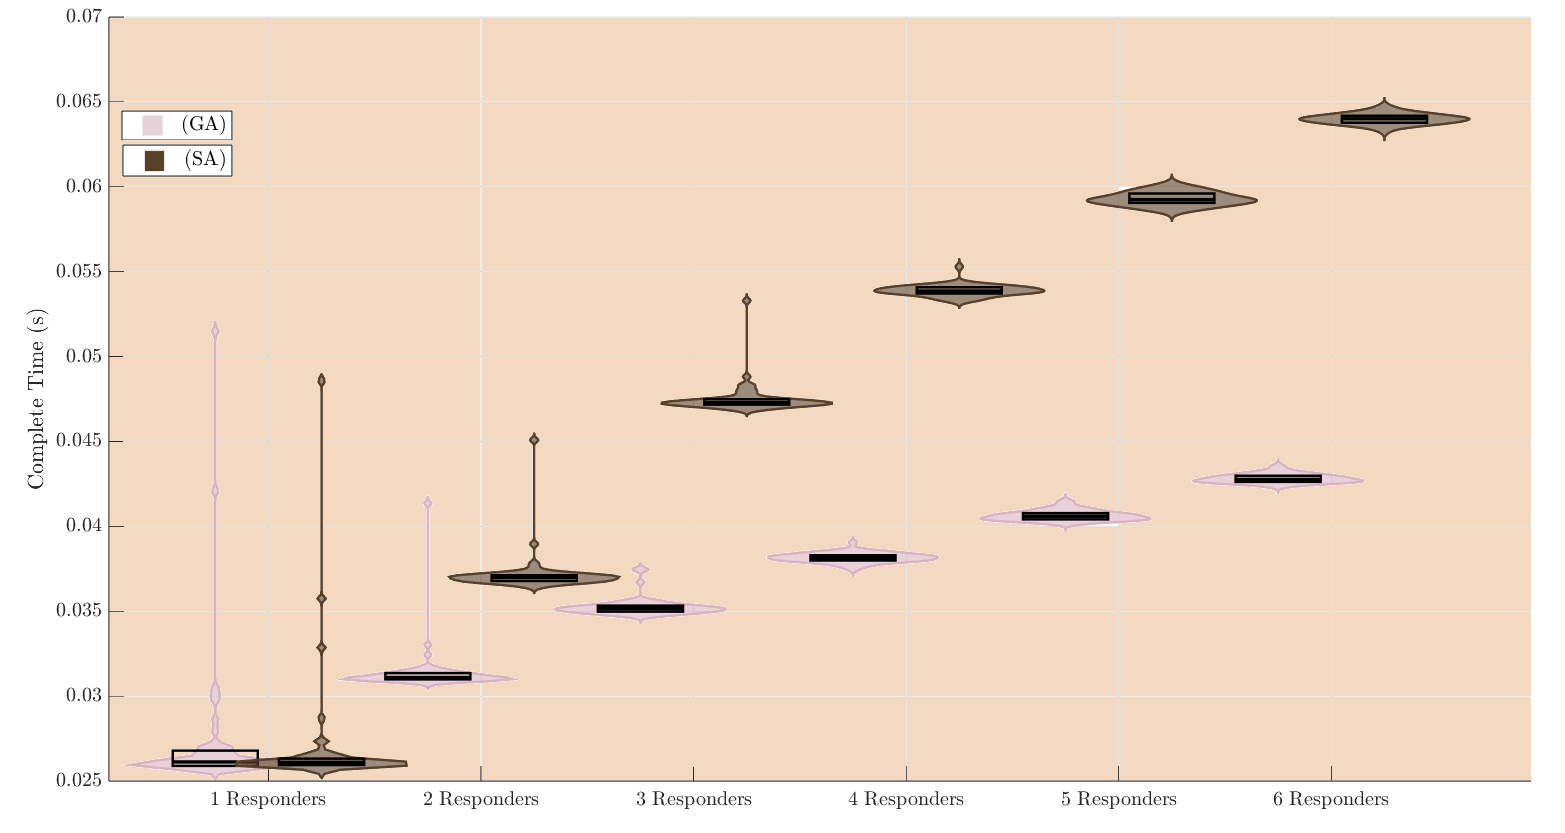
\includegraphics[width=0.95\linewidth]{fig/compare.png}
    \caption{Violin Plot of Algorithm Execution Time Distribution (100 Runs)}
    \label{fig:compare}
\end{figure}
Based on 100 repeated runs on different scenarios, the performance comparison between Genetic Algorithm (GA) and Simulated Annealing (SA) is as follows:

\begin{itemize}
    \item Runtime: In the scenario with 1 firefighter, SA is slightly faster than GA (2.3\% faster). However, as the number of firefighters increases (2-6), GA's time advantage gradually expands, from 19.2\% faster to 49.2\% faster. The average runtime of GA is 0.036 seconds, significantly lower than SA's 0.048 seconds. Both algorithms show small runtime fluctuations, with GA ranging from ±0.000 to ±0.003 seconds and SA from ±0.001 to ±0.003 seconds.
    \item Optimization quality: The fitness difference between the two algorithms is minimal (maximum gap of only 0.0002), with overall average fitness values being close (0.6805 for GA and 0.6804 for SA). GA's fitness fluctuation is more stable (±0.0000-0.0005), while SA's fluctuation ranges from ±0.0001-0.0007.
    \item GA: More advantageous in scenarios with more firefighters (2-6), with time advantages increasing as the scale expands and stable optimization quality.
    \item SA: Only shows a slight time advantage in simple scenarios with 1 firefighter, with fitness basically on par with GA.
\end{itemize}


